% Schematic curves from E:/网页下载/fig_response_threshold_band.tex.
\documentclass[tikz,border=2pt]{standalone}
\usepackage{fontspec}
\IfFontExistsTF{Times New Roman}{\setmainfont{Times New Roman}}{\setmainfont{Tinos}}
\usepackage{unicode-math}
\setmathfont{STIXTwoMath-Regular.otf}
\usetikzlibrary{arrows.meta}
\definecolor{ink}{HTML}{253139}
\definecolor{blueink}{HTML}{52758A}
\definecolor{linegray}{HTML}{65747E}
\definecolor{guidegray}{HTML}{AEBBC4}
\definecolor{framegray}{HTML}{C9D2D8}
\definecolor{safefill}{HTML}{D5E6F1}
\definecolor{overlapfill}{HTML}{F7E6AF}
\definecolor{intervalink}{HTML}{9B752B}
% Sizes refer to the standalone artwork, matching the restored partition figures
% after their respective inclusion scales. No body-size enlargement is applied.
\tikzset{
  font=\fontsize{12}{14.4}\selectfont,text=ink,
  labelsmall/.style={font=\fontsize{11.4}{13.7}\selectfont},
  axislabel/.style={font=\fontsize{12.8}{15.4}\selectfont},
  legend/.style={font=\fontsize{10.8}{13}\selectfont},
  axisarrow/.style={-{Stealth[length=4pt,width=4.3pt]},line width=.85pt,draw=ink},
  bound/.style={draw=blueink,line width=1.1pt},
  truecdf/.style={draw=ink,line width=.95pt,dash pattern=on 3.5pt off 2.5pt},
  guide/.style={draw=guidegray,line width=.45pt,densely dashed},
  leader/.style={draw=linegray,line width=.45pt,-{Stealth[length=3pt,width=3pt]}},
  interval/.style={draw=intervalink,line width=1.45pt}
}
\newcommand{\bandkey}{\tikz[baseline=2.3pt]{%
  \draw[fill=safefill,draw=blueink,line width=.6pt] (0,0) rectangle (10.5pt,9pt);}}
\newcommand{\cdfkey}{\tikz[baseline=-.45ex]{%
  \draw[truecdf] (0,0)--(16pt,0);}}
\newcommand{\intervalkey}{\tikz[baseline=2.6pt]{%
  \draw[interval] (0,0)--(0,10pt);
  \foreach \y in {0,10pt}
    \node[circle,draw=intervalink,fill=overlapfill,inner sep=0pt,minimum size=3.3pt,line width=.6pt] at (0,\y) {};}}

\begin{document}
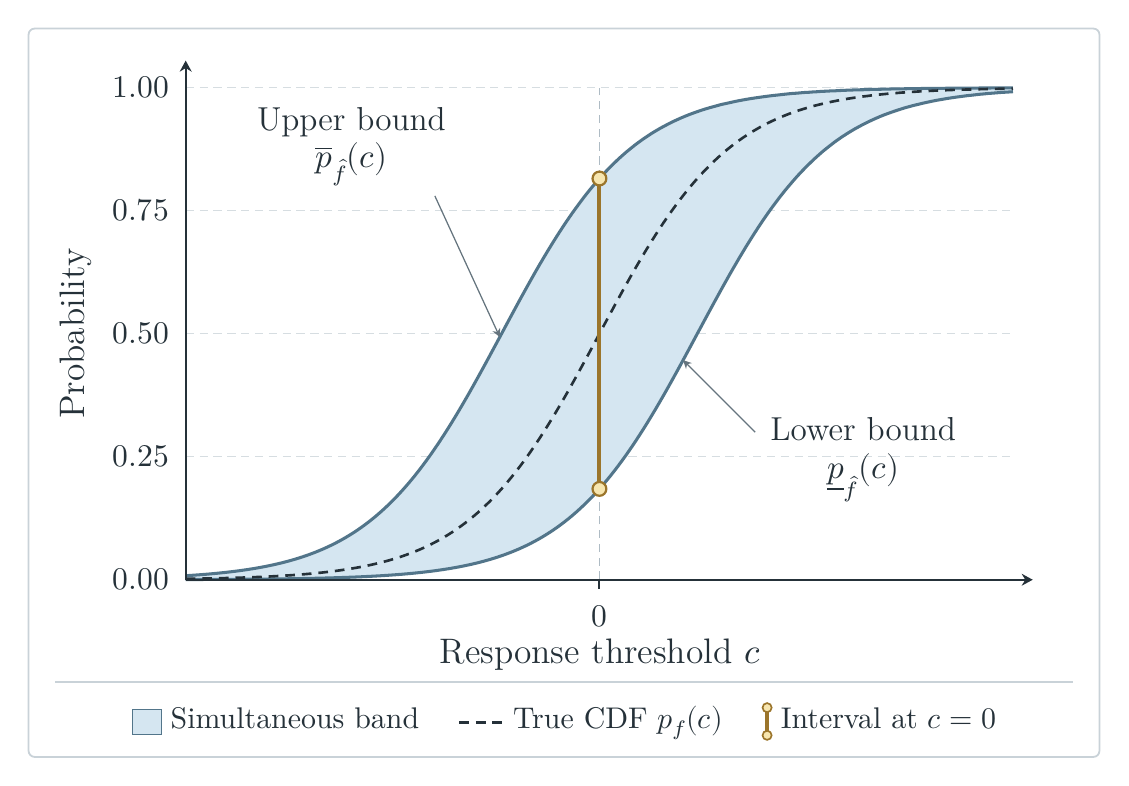
\begin{tikzpicture}[x=1cm,y=1cm]
  \draw[draw=framegray,line width=.65pt,rounded corners=2.2pt]
    (0,0) rectangle (13.6,9.25);
  % The supplied logistic functions and their horizontal shifts are preserved.
  \pgfmathdeclarefunction{uppercdf}{1}{\pgfmathparse{1/(1+exp(-1.35*(#1+1.1)))}}
  \pgfmathdeclarefunction{lowercdf}{1}{\pgfmathparse{1/(1+exp(-1.35*(#1-1.1)))}}
  \pgfmathdeclarefunction{truecdf}{1}{\pgfmathparse{1/(1+exp(-1.35*#1))}}
  \pgfmathsetmacro{\plo}{lowercdf(0)}
  \pgfmathsetmacro{\phi}{uppercdf(0)}
  \begin{scope}[shift={(7.25,2.25)},x=1.13cm,y=6.25cm]
    \foreach \p/\lab in {0/0.00,.25/0.25,.5/0.50,.75/0.75,1/1.00}{
      \draw[draw=guidegray!50,line width=.45pt,densely dashed] (-4.65,\p)--(4.65,\p);
      \node[anchor=east,labelsmall,inner sep=3pt] at (-4.74,\p) {$\lab$};
    }
    \fill[safefill]
      plot[domain=-4.65:4.65,samples=200] (\x,{uppercdf(\x)})
      -- plot[domain=4.65:-4.65,samples=200] (\x,{lowercdf(\x)}) -- cycle;
    \draw[guide] (0,0)--(0,1);
    \draw[bound] plot[domain=-4.65:4.65,samples=200] (\x,{uppercdf(\x)});
    \draw[bound] plot[domain=-4.65:4.65,samples=200] (\x,{lowercdf(\x)});
    \draw[truecdf] plot[domain=-4.65:4.65,samples=200] (\x,{truecdf(\x)});
    \draw[interval] (0,\plo)--(0,\phi);
    \foreach \p in {\plo,\phi}
      \node[circle,draw=intervalink,fill=overlapfill,inner sep=0pt,
        minimum size=5pt,line width=.8pt] at (0,\p) {};
    \draw[axisarrow] (-4.65,0)--(4.87,0);
    \draw[axisarrow] (-4.65,0)--(-4.65,1.055);
    \draw[ink,line width=.7pt] (0,0)--(0,-.018);
    \node[anchor=north,labelsmall,inner sep=3pt] at (0,-.035) {$0$};
    \draw[leader] (-1.85,.78)--(-1.12,{uppercdf(-1.12)});
    \draw[leader] (1.75,.30)--(.94,{lowercdf(.94)});
  \end{scope}
  \node[align=center,inner sep=0pt] at (4.10,7.75)
    {Upper bound\\[-1pt]$\overline p_{\hat f}(c)$};
  \node[align=center,inner sep=0pt] at (10.60,3.77)
    {Lower bound\\[-1pt]$\underline p_{\hat f}(c)$};
  \node[rotate=90,axislabel] at (.60,5.375) {Probability};
  \node[axislabel] at (7.25,1.30) {Response threshold $c$};
  \draw[draw=framegray,line width=.45pt] (.34,.95)--(13.26,.95);
  % Center the complete single-row legend, as in the restored figures.
  \node[legend,anchor=center,inner sep=0pt] at (6.80,.45) {%
    \bandkey\hspace{3pt}Simultaneous band\hspace{14pt}%
    \cdfkey\hspace{3pt}True CDF $p_f(c)$\hspace{14pt}%
    \intervalkey\hspace{3pt}Interval at $c=0$};
\end{tikzpicture}
\end{document}
